\chapter{Hopcroft's algorithm}

An automaton is \textit{accessible} when for any state $p\in Q$, there exists a word $w\in V^\ast$ such that $q_0\cdot w=p$. It is \textit{co-accessible} when for any state $p\in Q$, there exists $w\in V^\ast$ such that $p\cdot w\in F$.

\subsection{algorithm}

Member function min\_Hopcroft implements Hopcroft's $n\log n$ minimization algorithm, as presented in [\cite{WATSON94b}, Algorithm 4.8].

\begin{algorithm}  
	\caption{Hopcroft's minimization algorithm}  \label{alg:hopcroft}
	\begin{algorithmic}[1] %每行显示行号  
		\Require $G =(Q,V,T,q_0,F)$  
		\Ensure The equivalence classes of $Q$  
		\State $P \gets [Q]_{E_0}=\{F,Q\setminus F \}$  \qquad\qquad $\triangleright$ The initial partitions is $[Q]_{E_0}$, it's the total euivalence relation.
		
		\State $L \gets 0$  \qquad\qquad $\triangleright$ The waiting set
		
		\ForAll {$a\in V$}
			\State $ADD((min(F,Q\setminus F),a),L)$ \qquad\qquad 			$\triangleright$ initialization of the waiting set
		\EndFor
		\While {$L\ne\emptyset$}
			\State $P_{old} = P;$
			\State $(Q_1,a)\gets TakeSome(L)$ \qquad\qquad $\triangleright$ Take and remove some splitter
			\State $L=L\setminus \{(Q_1,a)\};$
			\ForAll {$Q_0\in P_{old} $}
				\State $Q_0$ is split by $(Q_1,a)$  \qquad\qquad $\triangleright$ Compute the split, $Q_0$ is splitted into $Q_0^\prime$ and $Q_0^{\prime\prime}$
				\State $Q_0^{\prime}=\{p|p\in Q_0\land T(p,a)\in Q_1\}$ 
				\State $Q_0^{\prime\prime}=\{Q_0\setminus Q_0^\prime\}$
				\State $P=P\setminus \{Q_0\}\cup\{Q_0^\prime, Q_0^{\prime\prime}\}$ \qquad\qquad $\triangleright$ Refine the partition, Replace $Q_0$ by $Q_0^\prime$ and $Q_0^{\prime\prime}$ in $P$.
			
				\ForAll {$b\in V$}  \qquad\qquad $\triangleright$ Update the waiting set
					\If {$(Q_0,b)\in L$}
						\State $L=L\setminus \{(Q_0,b)\}\cup\{(Q_0^\prime,b),(Q_0^{\prime\prime},b)\} $ \qquad\qquad $\triangleright$ Replace $(Q_0, b)$ by $(Q_0^\prime, b)$ and $(Q_0^{\prime\prime}, b)$ in $L$
					\Else
						\State $ADD((min(Q^\prime,Q^{\prime\prime}),b),L)$
						\EndIf  
				\EndFor
			\EndFor 
		\EndWhile
	\end{algorithmic}
\end{algorithm}

The combination of the out-transitions of all of the States is stored in a
\textbf{CRSet $C$}. 

Set \text{$L$} from the abstract algorithm is implemented as a mapping from States to int (an array of int is used). 

Array $L$ should be interpreted as follows: if State q a representative,
then the following pairs still require processing (are still in abstract set L):
$$([q], C_0),\cdots, ([q], C_{L(q)-1}) $$

The remaining pairs do not require processing:
$$([q], C_{L[q])}),\cdots, ([q], C_{|C|-1}) $$

This implementation facilitates quick scanning of $L$ for the next valid State-CharRange pair.

\begin{algorithm}[htbp]
	\caption{Hopcroft's minimization algorithm}  \label{alg:hopcroft}
	\begin{algorithmic}[1] %每行显示行号  
		\Require $G =(Q,V,T,q_0,F)$  
		\Ensure The equivalence classes of $Q$  
		\State $P \gets [Q]_{E_0}=\{F,Q\setminus F \}$  \qquad\qquad $\triangleright$ The initial partitions is $[Q]_{E_0}$, it's the total euivalence relation.
		
		\State $L \gets 0$  \qquad\qquad $\triangleright$ The waiting set
		\State $C = V$  \qquad\qquad $\triangleright$ C is all symbols set
		
		\If {$|F|\le |Q\setminus F|$}  \qquad\qquad 			$\triangleright$ initialization of the waiting set
			\State $L[q]=C.Size(), [q]$ is the representive of the $F$
		\Else
			\State $L[q]=C.Size(), [q]$ is the representive of the $Q\setminus F$
		\EndIf
		
		\While {(1)}
			\If {all L[q]=0 } 
				\State break;
			\EndIf
			
			\State Find the first pair in L that still needs processing. $(Q_1,a) = [q], L[q]\ne 0$ \qquad\qquad $\triangleright$ Take and remove some splitter
			
			\State $P_{old} = P$  \qquad\qquad $\triangleright$ current partitions
			
			\State $L[q]--$; \qquad\qquad $\triangleright$ Mark this element of L as processed.
	
			\ForAll {$Q_0\in P_{old} $}
				\State $Q_0$ is split by $(Q_1,a)$  \qquad\qquad $\triangleright$ Compute the split, $Q_0$ is splitted into $Q_0^\prime$ and $Q_0^{\prime\prime}$
				\State $Q_0^{\prime}=\{p|p\in Q_0\land T(p,a)\in Q_1\}$ 
				\State $Q_0^{\prime\prime}=\{Q_0\setminus Q_0^\prime\}$
				\State $P=P\setminus \{Q_0\}\cup\{Q_0^\prime, Q_0^{\prime\prime}\}$ \qquad\qquad $\triangleright$ Refine the partition, Replace $Q_0$ by $Q_0^\prime$ and $Q_0^{\prime\prime}$ in $P$.
				\State $p=Q_0$
				\State $r=Q_0^\prime$
				\If {$[r] != Invalid$}  \qquad\qquad $\triangleright$ Update the waiting set
					\If {($ [p]\le |[r]|$)}
					\State $L[r]=L[p] $ \qquad\qquad $\triangleright$  [r]待处理L[p]剩下的字符
					\State $L[p]=C.size()$  \qquad\qquad $\triangleright$  新的[p], 待处理C[0]...C[C.size()-1]
					\Else
					\State $L[r]=C.size() $ \qquad\qquad $\triangleright$ // 新的[r],待处理C[0]...C[C.size()-1]
					\EndIf  
				\EndIf 
			\EndFor
		\EndWhile
	\end{algorithmic}
\end{algorithm}

\subsection{Minimization example 1}

\begin{figure} [htbp]
	\centering 
	\subfigure[DFA,Eq class=\{\{4,5\},\{6,7\}\}] { %\label{fig:a2} 
		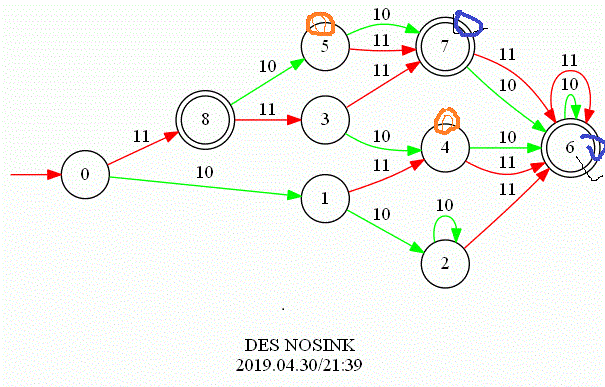
\includegraphics[width=0.4\columnwidth] {NOSINK} 
	} 
	\subfigure[mini-DFA] { %\label{fig:b2} 
		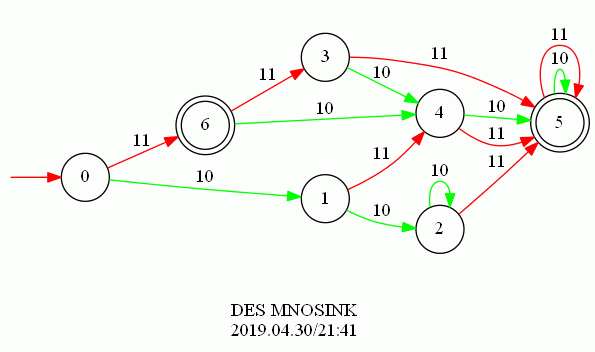
\includegraphics[width=0.4\columnwidth] {MNOSINK} 
	} 
	\caption{ Minimization example 1 } 
	\label{fig:mini-1} 
\end{figure}

CRSet C;  // the out labels of State's:{ 'a'  'b' } 

int L[9]: // the index of L = q: 对应等价类[q]; L[q]表示正在处理等价类[q]的字符在C中的index。$L = \{ 0,0,0,0,0,0,0,0,0 \} $

\begin{lstlisting}

DFA
Q = [0,9)
S = { 0 }
F = { 6  7  8 }
Transitions = 
0->{ 'a'->1  'b'->8 }
1->{ 'a'->2  'b'->4 }
2->{ 'a'->2  'b'->6 }
3->{ 'a'->4  'b'->7 }
4->{ ['a','b']->6 }
5->{ ['a','b']->7 }
6->{ ['a','b']->6 }
7->{ ['a','b']->6 }
8->{ 'a'->5  'b'->3 }

current = -1

is the DFA Usefulf ?: 1

The combination for all the out labels of State's:C = { 'a'  'b' }
L:
0 1 2 3 4 5 6 7 8
0 0 0 0 0 0 0 0 0
Initialize partitions, E0:
StateEqRel
{ 0  1  2  3  4  5 }
{ 6  7  8 }

Initialize L repr = {F}:
{ 6 }
L:
0 1 2 3 4 5 6 7 8
0 0 0 0 0 0 2 0 0
=========================== Iterate: k = 1
L:
0 1 2 3 4 5 6 7 8
0 0 0 0 0 0 1 0 0
Partitions:
StateEqRel
{ 0  1  2  3  4  5 }
{ 6  7  8 }

pick [q] in L:([q],a)=([6],'b')
split [p] w.r.t ([6],'b')
===split[0] w.r.t ([6],'b')
new split of [0] is [1]
[p]={ 0  2  3  4  5 }
[r]={ 1 }
p and r are the new representatives. Now update L with the smallest of [0] and [1]
using [r] = [1],L[r]=C.size();
after update L: 
L:
0 1 2 3 4 5 6 7 8
0 2 0 0 0 0 1 0 0
===split[6] w.r.t ([6],'b')
new split of [6] is [8]
[p]={ 6  7 }
[r]={ 8 }
p and r are the new representatives. Now update L with the smallest of [6] and [8]
using [r] = [8],L[r]=C.size();
after update L: 
L:
0 1 2 3 4 5 6 7 8
0 2 0 0 0 0 1 0 2
=========================== Iterate: k = 2
L:
0 1 2 3 4 5 6 7 8
0 1 0 0 0 0 1 0 2
Partitions:
StateEqRel
{ 0  2  3  4  5 }
{ 1 }
{ 6  7 }
{ 8 }

pick [q] in L:([q],a)=([1],'b')
split [p] w.r.t ([1],'b')
===split[0] w.r.t ([1],'b')
new split of [0] is [-1]
===split[1] w.r.t ([1],'b')
new split of [1] is [-1]
===split[6] w.r.t ([1],'b')
new split of [6] is [-1]
===split[8] w.r.t ([1],'b')
new split of [8] is [-1]
=========================== Iterate: k = 3
L:
0 1 2 3 4 5 6 7 8
0 0 0 0 0 0 1 0 2
Partitions:
StateEqRel
{ 0  2  3  4  5 }
{ 1 }
{ 6  7 }
{ 8 }

pick [q] in L:([q],a)=([1],'a')
split [p] w.r.t ([1],'a')
===split[0] w.r.t ([1],'a')
new split of [0] is [2]
[p]={ 0 }
[r]={ 2  3  4  5 }
p and r are the new representatives. Now update L with the smallest of [0] and [2]
using [p] = [0],L[r]=L[p]; L[p]=C.size();
after update L: 
L:
0 1 2 3 4 5 6 7 8
2 0 0 0 0 0 1 0 2
===split[1] w.r.t ([1],'a')
new split of [1] is [-1]
===split[6] w.r.t ([1],'a')
new split of [6] is [-1]
===split[8] w.r.t ([1],'a')
new split of [8] is [-1]
=========================== Iterate: k = 4
L:
0 1 2 3 4 5 6 7 8
1 0 0 0 0 0 1 0 2
Partitions:
StateEqRel
{ 0 }
{ 1 }
{ 2  3  4  5 }
{ 6  7 }
{ 8 }

pick [q] in L:([q],a)=([0],'b')
split [p] w.r.t ([0],'b')
===split[0] w.r.t ([0],'b')
new split of [0] is [-1]
===split[1] w.r.t ([0],'b')
new split of [1] is [-1]
===split[2] w.r.t ([0],'b')
new split of [2] is [-1]
===split[6] w.r.t ([0],'b')
new split of [6] is [-1]
===split[8] w.r.t ([0],'b')
new split of [8] is [-1]
=========================== Iterate: k = 5
L:
0 1 2 3 4 5 6 7 8
0 0 0 0 0 0 1 0 2
Partitions:
StateEqRel
{ 0 }
{ 1 }
{ 2  3  4  5 }
{ 6  7 }
{ 8 }

pick [q] in L:([q],a)=([0],'a')
split [p] w.r.t ([0],'a')
===split[0] w.r.t ([0],'a')
new split of [0] is [-1]
===split[1] w.r.t ([0],'a')
new split of [1] is [-1]
===split[2] w.r.t ([0],'a')
new split of [2] is [-1]
===split[6] w.r.t ([0],'a')
new split of [6] is [-1]
===split[8] w.r.t ([0],'a')
new split of [8] is [-1]
=========================== Iterate: k = 6
L:
0 1 2 3 4 5 6 7 8
0 0 0 0 0 0 0 0 2
Partitions:
StateEqRel
{ 0 }
{ 1 }
{ 2  3  4  5 }
{ 6  7 }
{ 8 }

pick [q] in L:([q],a)=([6],'a')
split [p] w.r.t ([6],'a')
===split[0] w.r.t ([6],'a')
new split of [0] is [-1]
===split[1] w.r.t ([6],'a')
new split of [1] is [-1]
===split[2] w.r.t ([6],'a')
new split of [2] is [4]
[p]={ 2  3 }
[r]={ 4  5 }
p and r are the new representatives. Now update L with the smallest of [2] and [4]
using [p] = [2],L[r]=L[p]; L[p]=C.size();
after update L: 
L:
0 1 2 3 4 5 6 7 8
0 0 2 0 0 0 0 0 2
===split[6] w.r.t ([6],'a')
new split of [6] is [-1]
===split[8] w.r.t ([6],'a')
new split of [8] is [-1]
=========================== Iterate: k = 7
L:
0 1 2 3 4 5 6 7 8
0 0 1 0 0 0 0 0 2
Partitions:
StateEqRel
{ 0 }
{ 1 }
{ 2  3 }
{ 4  5 }
{ 6  7 }
{ 8 }

pick [q] in L:([q],a)=([2],'b')
split [p] w.r.t ([2],'b')
===split[0] w.r.t ([2],'b')
new split of [0] is [-1]
===split[1] w.r.t ([2],'b')
new split of [1] is [-1]
===split[2] w.r.t ([2],'b')
new split of [2] is [-1]
===split[4] w.r.t ([2],'b')
new split of [4] is [-1]
===split[6] w.r.t ([2],'b')
new split of [6] is [-1]
===split[8] w.r.t ([2],'b')
new split of [8] is [-1]
=========================== Iterate: k = 8
L:
0 1 2 3 4 5 6 7 8
0 0 0 0 0 0 0 0 2
Partitions:
StateEqRel
{ 0 }
{ 1 }
{ 2  3 }
{ 4  5 }
{ 6  7 }
{ 8 }

pick [q] in L:([q],a)=([2],'a')
split [p] w.r.t ([2],'a')
===split[0] w.r.t ([2],'a')
new split of [0] is [-1]
===split[1] w.r.t ([2],'a')
new split of [1] is [-1]
===split[2] w.r.t ([2],'a')
new split of [2] is [3]
[p]={ 2 }
[r]={ 3 }
p and r are the new representatives. Now update L with the smallest of [2] and [3]
using [p] = [2],L[r]=L[p]; L[p]=C.size();
after update L: 
L:
0 1 2 3 4 5 6 7 8
0 0 2 0 0 0 0 0 2
===split[4] w.r.t ([2],'a')
new split of [4] is [-1]
===split[6] w.r.t ([2],'a')
new split of [6] is [-1]
===split[8] w.r.t ([2],'a')
new split of [8] is [-1]
=========================== Iterate: k = 9
L:
0 1 2 3 4 5 6 7 8
0 0 1 0 0 0 0 0 2
Partitions:
StateEqRel
{ 0 }
{ 1 }
{ 2 }
{ 3 }
{ 4  5 }
{ 6  7 }
{ 8 }

pick [q] in L:([q],a)=([2],'b')
split [p] w.r.t ([2],'b')
===split[0] w.r.t ([2],'b')
new split of [0] is [-1]
===split[1] w.r.t ([2],'b')
new split of [1] is [-1]
===split[2] w.r.t ([2],'b')
new split of [2] is [-1]
===split[3] w.r.t ([2],'b')
new split of [3] is [-1]
===split[4] w.r.t ([2],'b')
new split of [4] is [-1]
===split[6] w.r.t ([2],'b')
new split of [6] is [-1]
===split[8] w.r.t ([2],'b')
new split of [8] is [-1]
=========================== Iterate: k = 10
L:
0 1 2 3 4 5 6 7 8
0 0 0 0 0 0 0 0 2
Partitions:
StateEqRel
{ 0 }
{ 1 }
{ 2 }
{ 3 }
{ 4  5 }
{ 6  7 }
{ 8 }

pick [q] in L:([q],a)=([2],'a')
split [p] w.r.t ([2],'a')
===split[0] w.r.t ([2],'a')
new split of [0] is [-1]
===split[1] w.r.t ([2],'a')
new split of [1] is [-1]
===split[2] w.r.t ([2],'a')
new split of [2] is [-1]
===split[3] w.r.t ([2],'a')
new split of [3] is [-1]
===split[4] w.r.t ([2],'a')
new split of [4] is [-1]
===split[6] w.r.t ([2],'a')
new split of [6] is [-1]
===split[8] w.r.t ([2],'a')
new split of [8] is [-1]
=========================== Iterate: k = 11
L:
0 1 2 3 4 5 6 7 8
0 0 0 0 0 0 0 0 1
Partitions:
StateEqRel
{ 0 }
{ 1 }
{ 2 }
{ 3 }
{ 4  5 }
{ 6  7 }
{ 8 }

pick [q] in L:([q],a)=([8],'b')
split [p] w.r.t ([8],'b')
===split[0] w.r.t ([8],'b')
new split of [0] is [-1]
===split[1] w.r.t ([8],'b')
new split of [1] is [-1]
===split[2] w.r.t ([8],'b')
new split of [2] is [-1]
===split[3] w.r.t ([8],'b')
new split of [3] is [-1]
===split[4] w.r.t ([8],'b')
new split of [4] is [-1]
===split[6] w.r.t ([8],'b')
new split of [6] is [-1]
===split[8] w.r.t ([8],'b')
new split of [8] is [-1]
=========================== Iterate: k = 12
L:
0 1 2 3 4 5 6 7 8
0 0 0 0 0 0 0 0 0
Partitions:
StateEqRel
{ 0 }
{ 1 }
{ 2 }
{ 3 }
{ 4  5 }
{ 6  7 }
{ 8 }

pick [q] in L:([q],a)=([8],'a')
split [p] w.r.t ([8],'a')
===split[0] w.r.t ([8],'a')
new split of [0] is [-1]
===split[1] w.r.t ([8],'a')
new split of [1] is [-1]
===split[2] w.r.t ([8],'a')
new split of [2] is [-1]
===split[3] w.r.t ([8],'a')
new split of [3] is [-1]
===split[4] w.r.t ([8],'a')
new split of [4] is [-1]
===split[6] w.r.t ([8],'a')
new split of [6] is [-1]
===split[8] w.r.t ([8],'a')
new split of [8] is [-1]

************ minDFA

DFA
Q = [0,7)
S = { 0 }
F = { 5  6 }
Transitions = 
0->{ 'a'->1  'b'->6 }
1->{ 'a'->2  'b'->4 }
2->{ 'a'->2  'b'->5 }
3->{ 'a'->4  'b'->5 }
4->{ ['a','b']->5 }
5->{ ['a','b']->5 }
6->{ 'a'->4  'b'->3 }

current = -1

\end{lstlisting}


\section{Minimization example 2}

\begin{figure}[htbp]
	\begin{tikzpicture}[->,>=stealth',shorten >=1pt,auto,node distance=2cm, semithick]
	\tikzstyle{every state}=[minimum size=0.1mm]
	
	\node[initial,state] (q0)  {$q_0$};
	\node[state]         (q1) [right of=q0] {$q_1$};
	\node[state,accepting]         (q2) [below of=q0] {$q_2$};
	\node[state,accepting]         (q3) [below of=q1] {$q_3$};
	\node[state,accepting]         (q4) [below of=q2] {$q_4$};
	\node[state]         (q5) [below of=q3] {$q_5$};
	\path 
	(q0) edge [bend left]       node {0} (q1)
	     edge                   node {1} (q2)
	(q1) edge [bend left]       node {0} (q0)
	     edge                   node {1} (q3)
	(q2) edge                   node {0} (q4)
		 edge                   node {1} (q5)
	(q3) edge                   node {0} (q4)
	     edge                   node {1} (q5)
	(q4) edge                   node {1} (q5)
	     edge [loop left]       node {0} (q4)
	(q5) edge [loop right]      node {0,1} (q5)
	;
	\end{tikzpicture}
	\caption{Minimization example 2}
\end{figure}

\begin{lstlisting}
	DFA
	Q = [0,6)
	S = { 0 }
	F = { 2  3  4 }
	Transitions = 
	0->{ '0'->1  '1'->2 }
	1->{ '0'->0  '1'->3 }
	2->{ '0'->4  '1'->5 }
	3->{ '0'->4  '1'->5 }
	4->{ '0'->4  '1'->5 }
	5->{ ['0','1']->5 }
	
	current = -1
	
	is the DFA Usefulf ?: 0
	
	The combination for all the out labels of State's:C = { '0'  '1' }
	L:
	0 1 2 3 4 5
	0 0 0 0 0 0
	Initialize partitions, E0:
	StateEqRel
	{ 0  1  5 }
	{ 2  3  4 }
	
	Initialize L repr = {F}:
	{ 2 }
	L:
	0 1 2 3 4 5
	0 0 2 0 0 0
	=========================== Iterate: k = 1
	L:
	0 1 2 3 4 5
	0 0 1 0 0 0
	Partitions:
	StateEqRel
	{ 0  1  5 }
	{ 2  3  4 }
	
	pick [q] in L:([q],a)=([2],'1')
	split [p] w.r.t ([2],'1')
	===split[0] w.r.t ([2],'1')
	new split of [0] is [5]
	[p]={ 0  1 }
	[r]={ 5 }
	p and r are the new representatives. Now update L with the smallest of [0] and [5]
	using [r] = [5],L[r]=C.size();
	after update L: 
	L:
	0 1 2 3 4 5
	0 0 1 0 0 2
	===split[2] w.r.t ([2],'1')
	new split of [2] is [-1]
	=========================== Iterate: k = 2
	L:
	0 1 2 3 4 5
	0 0 0 0 0 2
	Partitions:
	StateEqRel
	{ 0  1 }
	{ 2  3  4 }
	{ 5 }
	
	pick [q] in L:([q],a)=([2],'0')
	split [p] w.r.t ([2],'0')
	===split[0] w.r.t ([2],'0')
	new split of [0] is [-1]
	===split[2] w.r.t ([2],'0')
	new split of [2] is [-1]
	===split[5] w.r.t ([2],'0')
	new split of [5] is [-1]
	=========================== Iterate: k = 3
	L:
	0 1 2 3 4 5
	0 0 0 0 0 1
	Partitions:
	StateEqRel
	{ 0  1 }
	{ 2  3  4 }
	{ 5 }
	
	pick [q] in L:([q],a)=([5],'1')
	split [p] w.r.t ([5],'1')
	===split[0] w.r.t ([5],'1')
	new split of [0] is [-1]
	===split[2] w.r.t ([5],'1')
	new split of [2] is [-1]
	===split[5] w.r.t ([5],'1')
	new split of [5] is [-1]
	=========================== Iterate: k = 4
	L:
	0 1 2 3 4 5
	0 0 0 0 0 0
	Partitions:
	StateEqRel
	{ 0  1 }
	{ 2  3  4 }
	{ 5 }
	
	pick [q] in L:([q],a)=([5],'0')
	split [p] w.r.t ([5],'0')
	===split[0] w.r.t ([5],'0')
	new split of [0] is [-1]
	===split[2] w.r.t ([5],'0')
	new split of [2] is [-1]
	===split[5] w.r.t ([5],'0')
	new split of [5] is [-1]
	
	************ minDFA
	
	DFA
	Q = [0,3)
	S = { 0 }
	F = { 1 }
	Transitions = 
	0->{ '0'->0  '1'->1 }
	1->{ '0'->1  '1'->2 }
	2->{ ['0','1']->2 }
	
	current = -1
\end{list}

\end{lstlisting}
\section{Minimization example 3 ($1\to 2\to 3\to 4\to 5\to 6$)}

\begin{figure}[htbp]
	\begin{tikzpicture}[->,>=stealth',shorten >=1pt,auto,node distance=2cm, semithick]
	\tikzstyle{every state}=[minimum size=0.1mm]
	\node[initial,state] (p1)  {$0$};
	\node[state]         (p2) [right of=p1] {$1$};
	\node[state]         (p3) [right of=p2] {$2$};
	\node[state]         (p4) [right of=p3] {$3$};
	\node[state]         (p5) [right of=p4] {$4$};
	\node[state,accepting] (p6) [right of=p5] {$5$};
	\path
	(p1) edge [loop above] node {1} (p1)
	     edge [] node {0} (p2)
	(p2) edge [loop above] node {1} (p2)
	     edge [] node {0} (p3)
	(p3) edge [loop above] node {1} (p3)
		 edge [] node {0} (p4)
    (p4) edge [loop above] node {1} (p4)
         edge [] node {0} (p5)
    (p5) edge [loop above] node {1} (p5)
         edge [] node {0} (p6)
    (p6) edge [loop above] node {0,1} (p6)
	;
	\end{tikzpicture}
	\caption{Minimizing example} \label{fig:mini-ex1}
\end{figure}

split $Q_0$ w.r.t. ($Q_1,0$), see Fig. \ref{fig:split}.

Ex 1: $Q_0=\{0,1,2,3,4\}, Q_1=\{5\}$

Since, $Q_0^{\prime}=\{4\} \subseteq Q_0\text{, and }T(Q_0^{\prime},0) = T(\{4\},0)= {5}\in Q_1$ \\
$Q_0^{\prime\prime}=Q_0\setminus Q_0^\prime=\{0,1,2,3\}\subseteq Q_0\text{, and }T(Q_0^{\prime\prime},0) = T(\{0,1,2,3\},0)=T(\{0\},0)\cup T(\{1\},0)\cup T(\{2\},0)\cup T(\{3\},0) = \{1\} \cup \{2\} \cup \{3\} =\{1,2,3\}\notin Q_1$ 

$\therefore$
$Q_0$ w.r.t. ($Q_1,0$) is splitted into two parts. part(1) $Q_0^\prime=\{4\}$, part(2) $Q_0^{\prime\prime}=Q_0\setminus Q_0^\prime=\{0,1,2,3\}$ 
\newline

Ex 2: $Q_0=\{5\}, Q_1=\{0,1,2,3,4\}$

Since, $\forall q\in Q_0,\nexists T(q,a)\in Q_1$

$\therefore$
$Q_0$ w.r.t. ($Q_1,0$) 是一个无效的split, 同样$Q_0=Q_1=\{5\}$也是一个无效的split。
\newline

Ex 3: $Q_0=\{0,1,2,3,4\}, Q_1=\{0,1,2,3,4\}$

Since, $Q_0^{\prime}=\{0,1,2,3\}\subseteq Q_0\text{, and }T(Q_0^{\prime},0) = T(\{0,1,2,3\},0)=T(\{0\},0)\cup T(\{1\},0)\cup T(\{2\},0)\cup T(\{3\},0) = \{1\} \cup \{2\} \cup \{3\} =\{1,2,3\}\in Q_1$ \\
$Q_0^{\prime\prime}=Q_0\setminus Q_0^\prime=\{4\}\subseteq Q_0\text{, and }T(Q_0^{\prime\prime},0) = T(\{4\},0)= {5}\notin Q_1$ 

$\therefore$
$Q_0$ w.r.t. ($Q_1,0$) is splitted into two parts. part(1) $Q_0^\prime=\{0,1,2,3\}$, part(2) $Q_0^{\prime\prime}=Q_0\setminus Q_0^\prime=\{4\}$

\begin{figure}[htbp]
	if ($\exists p,q\in Q_0,T(p,a)\in Q_1$, and  $T(q,a)\notin Q_1$), then \\
	split $Q_0$ w.r.t. ($Q_1,a$) $\to$ two parts, (1): $Q_0^\prime\in Q_1$ and (2):
	 $(Q_0\setminus Q_0^\prime)\notin Q_1$ \\
	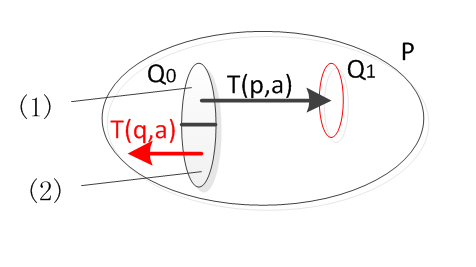
\includegraphics[scale=0.8]{splittable}
	\caption{split $Q_0$ w.r.t. ($Q_1,a$) }
	\label{fig:split}
\end{figure}


开始于:$[q]=\{Q\setminus F\} = \{0,1,2,3,4\}$, split [p] w.r.t ([q],a)

\begin{lstlisting}

************ DFA
DFA
Q = [0,6)
S = { 0 }
F = { 5 }
Transitions = 
0->{ '0'->1  '1'->0 }
1->{ '0'->2  '1'->1 }
2->{ '0'->3  '1'->2 }
3->{ '0'->4  '1'->3 }
4->{ '0'->5  '1'->4 }
5->{ ['0','1']->5 }

current = -1

is the DFA Usefulf ?: 1

The combination for all the out labels of State's:C = { '0'  '1' }
L:
0 1 2 3 4 5
0 0 0 0 0 0
Initialize partitions, E0:
StateEqRel
{ 0  1  2  3  4 }
{ 5 }

L:
0 1 2 3 4 5
2 0 0 0 0 0
=========================== Iterate: k = 1
L:
0 1 2 3 4 5
1 0 0 0 0 0
Partitions:
StateEqRel
{ 0  1  2  3  4 }
{ 5 }

pick [q] in L:([q],a)=([0],'1')
split [p] w.r.t ([0],'1')
===split[0] w.r.t ([0],'1')
new split of [0] is [-1]
===split[5] w.r.t ([0],'1')
new split of [5] is [-1]
=========================== Iterate: k = 2
L:
0 1 2 3 4 5
0 0 0 0 0 0
Partitions:
StateEqRel
{ 0  1  2  3  4 }
{ 5 }

pick [q] in L:([q],a)=([0],'0')
split [p] w.r.t ([0],'0')
===split[0] w.r.t ([0],'0')
new split of [0] is [4]
[p]={ 0  1  2  3 }
[r]={ 4 }
p and r are the new representatives. Now update L with the smallest of [0] and [4]
using [r] = [4],L[r]=C.size();
after update L: 
L:
0 1 2 3 4 5
0 0 0 0 2 0
===split[5] w.r.t ([0],'0')
new split of [5] is [-1]
=========================== Iterate: k = 3
L:
0 1 2 3 4 5
0 0 0 0 1 0
Partitions:
StateEqRel
{ 0  1  2  3 }
{ 4 }
{ 5 }

pick [q] in L:([q],a)=([4],'1')
split [p] w.r.t ([4],'1')
===split[0] w.r.t ([4],'1')
new split of [0] is [-1]
===split[4] w.r.t ([4],'1')
new split of [4] is [-1]
===split[5] w.r.t ([4],'1')
new split of [5] is [-1]
=========================== Iterate: k = 4
L:
0 1 2 3 4 5
0 0 0 0 0 0
Partitions:
StateEqRel
{ 0  1  2  3 }
{ 4 }
{ 5 }

pick [q] in L:([q],a)=([4],'0')
split [p] w.r.t ([4],'0')
===split[0] w.r.t ([4],'0')
new split of [0] is [3]
[p]={ 0  1  2 }
[r]={ 3 }
p and r are the new representatives. Now update L with the smallest of [0] and [3]
using [r] = [3],L[r]=C.size();
after update L: 
L:
0 1 2 3 4 5
0 0 0 2 0 0
===split[4] w.r.t ([4],'0')
new split of [4] is [-1]
===split[5] w.r.t ([4],'0')
new split of [5] is [-1]
=========================== Iterate: k = 5
L:
0 1 2 3 4 5
0 0 0 1 0 0
Partitions:
StateEqRel
{ 0  1  2 }
{ 3 }
{ 4 }
{ 5 }

pick [q] in L:([q],a)=([3],'1')
split [p] w.r.t ([3],'1')
===split[0] w.r.t ([3],'1')
new split of [0] is [-1]
===split[3] w.r.t ([3],'1')
new split of [3] is [-1]
===split[4] w.r.t ([3],'1')
new split of [4] is [-1]
===split[5] w.r.t ([3],'1')
new split of [5] is [-1]
=========================== Iterate: k = 6
L:
0 1 2 3 4 5
0 0 0 0 0 0
Partitions:
StateEqRel
{ 0  1  2 }
{ 3 }
{ 4 }
{ 5 }

pick [q] in L:([q],a)=([3],'0')
split [p] w.r.t ([3],'0')
===split[0] w.r.t ([3],'0')
new split of [0] is [2]
[p]={ 0  1 }
[r]={ 2 }
p and r are the new representatives. Now update L with the smallest of [0] and [2]
using [r] = [2],L[r]=C.size();
after update L: 
L:
0 1 2 3 4 5
0 0 2 0 0 0
===split[3] w.r.t ([3],'0')
new split of [3] is [-1]
===split[4] w.r.t ([3],'0')
new split of [4] is [-1]
===split[5] w.r.t ([3],'0')
new split of [5] is [-1]
=========================== Iterate: k = 7
L:
0 1 2 3 4 5
0 0 1 0 0 0
Partitions:
StateEqRel
{ 0  1 }
{ 2 }
{ 3 }
{ 4 }
{ 5 }

pick [q] in L:([q],a)=([2],'1')
split [p] w.r.t ([2],'1')
===split[0] w.r.t ([2],'1')
new split of [0] is [-1]
===split[2] w.r.t ([2],'1')
new split of [2] is [-1]
===split[3] w.r.t ([2],'1')
new split of [3] is [-1]
===split[4] w.r.t ([2],'1')
new split of [4] is [-1]
===split[5] w.r.t ([2],'1')
new split of [5] is [-1]
=========================== Iterate: k = 8
L:
0 1 2 3 4 5
0 0 0 0 0 0
Partitions:
StateEqRel
{ 0  1 }
{ 2 }
{ 3 }
{ 4 }
{ 5 }

pick [q] in L:([q],a)=([2],'0')
split [p] w.r.t ([2],'0')
===split[0] w.r.t ([2],'0')
new split of [0] is [1]
[p]={ 0 }
[r]={ 1 }
p and r are the new representatives. Now update L with the smallest of [0] and [1]
using [p] = [0],L[r]=L[p]; L[p]=C.size();
after update L: 
L:
0 1 2 3 4 5
2 0 0 0 0 0
===split[2] w.r.t ([2],'0')
new split of [2] is [-1]
===split[3] w.r.t ([2],'0')
new split of [3] is [-1]
===split[4] w.r.t ([2],'0')
new split of [4] is [-1]
===split[5] w.r.t ([2],'0')
new split of [5] is [-1]
=========================== Iterate: k = 9
L:
0 1 2 3 4 5
1 0 0 0 0 0
Partitions:
StateEqRel
{ 0 }
{ 1 }
{ 2 }
{ 3 }
{ 4 }
{ 5 }

pick [q] in L:([q],a)=([0],'1')
split [p] w.r.t ([0],'1')
===split[0] w.r.t ([0],'1')
new split of [0] is [-1]
===split[1] w.r.t ([0],'1')
new split of [1] is [-1]
===split[2] w.r.t ([0],'1')
new split of [2] is [-1]
===split[3] w.r.t ([0],'1')
new split of [3] is [-1]
===split[4] w.r.t ([0],'1')
new split of [4] is [-1]
===split[5] w.r.t ([0],'1')
new split of [5] is [-1]
=========================== Iterate: k = 10
L:
0 1 2 3 4 5
0 0 0 0 0 0
Partitions:
StateEqRel
{ 0 }
{ 1 }
{ 2 }
{ 3 }
{ 4 }
{ 5 }

pick [q] in L:([q],a)=([0],'0')
split [p] w.r.t ([0],'0')
===split[0] w.r.t ([0],'0')
new split of [0] is [-1]
===split[1] w.r.t ([0],'0')
new split of [1] is [-1]
===split[2] w.r.t ([0],'0')
new split of [2] is [-1]
===split[3] w.r.t ([0],'0')
new split of [3] is [-1]
===split[4] w.r.t ([0],'0')
new split of [4] is [-1]
===split[5] w.r.t ([0],'0')
new split of [5] is [-1]

************ minDFA

DFA
Q = [0,6)
S = { 0 }
F = { 5 }
Transitions = 
0->{ '0'->1  '1'->0 }
1->{ '0'->2  '1'->1 }
2->{ '0'->3  '1'->2 }
3->{ '0'->4  '1'->3 }
4->{ '0'->5  '1'->4 }
5->{ ['0','1']->5 }

current = -1

\end{lstlisting}

开始于:$[q]=\{F\} = \{5\}$, split [p] w.r.t. ([q],a)

\begin{lstlisting}

************ DFA

DFA
Q = [0,6)
S = { 0 }
F = { 5 }
Transitions = 
0->{ '0'->1  '1'->0 }
1->{ '0'->2  '1'->1 }
2->{ '0'->3  '1'->2 }
3->{ '0'->4  '1'->3 }
4->{ '0'->5  '1'->4 }
5->{ ['0','1']->5 }

current = -1

is the DFA Usefulf ?: 1

The combination for all the out labels of State's:C = { '0'  '1' }
L:
0 1 2 3 4 5
0 0 0 0 0 0
Initialize partitions, E0:
StateEqRel
{ 0  1  2  3  4 }
{ 5 }

Initialize L repr = {F}:
{ 5 }
L:
0 1 2 3 4 5
0 0 0 0 0 2
=========================== Iterate: k = 1
L:
0 1 2 3 4 5
0 0 0 0 0 1
Partitions:
StateEqRel
{ 0  1  2  3  4 }
{ 5 }

pick [q] in L:([q],a)=([5],'1')
split [p] w.r.t ([5],'1')
===split[0] w.r.t ([5],'1')
new split of [0] is [-1]
===split[5] w.r.t ([5],'1')
new split of [5] is [-1]
=========================== Iterate: k = 2
L:
0 1 2 3 4 5
0 0 0 0 0 0
Partitions:
StateEqRel
{ 0  1  2  3  4 }
{ 5 }

pick [q] in L:([q],a)=([5],'0')
split [p] w.r.t ([5],'0')
===split[0] w.r.t ([5],'0')
new split of [0] is [4]
[p]={ 0  1  2  3 }
[r]={ 4 }
p and r are the new representatives. Now update L with the smallest of [0] and [4]
using [r] = [4],L[r]=C.size();
after update L: 
L:
0 1 2 3 4 5
0 0 0 0 2 0
===split[5] w.r.t ([5],'0')
new split of [5] is [-1]
=========================== Iterate: k = 3
L:
0 1 2 3 4 5
0 0 0 0 1 0
Partitions:
StateEqRel
{ 0  1  2  3 }
{ 4 }
{ 5 }

pick [q] in L:([q],a)=([4],'1')
split [p] w.r.t ([4],'1')
===split[0] w.r.t ([4],'1')
new split of [0] is [-1]
===split[4] w.r.t ([4],'1')
new split of [4] is [-1]
===split[5] w.r.t ([4],'1')
new split of [5] is [-1]
=========================== Iterate: k = 4
L:
0 1 2 3 4 5
0 0 0 0 0 0
Partitions:
StateEqRel
{ 0  1  2  3 }
{ 4 }
{ 5 }

pick [q] in L:([q],a)=([4],'0')
split [p] w.r.t ([4],'0')
===split[0] w.r.t ([4],'0')
new split of [0] is [3]
[p]={ 0  1  2 }
[r]={ 3 }
p and r are the new representatives. Now update L with the smallest of [0] and [3]
using [r] = [3],L[r]=C.size();
after update L: 
L:
0 1 2 3 4 5
0 0 0 2 0 0
===split[4] w.r.t ([4],'0')
new split of [4] is [-1]
===split[5] w.r.t ([4],'0')
new split of [5] is [-1]
=========================== Iterate: k = 5
L:
0 1 2 3 4 5
0 0 0 1 0 0
Partitions:
StateEqRel
{ 0  1  2 }
{ 3 }
{ 4 }
{ 5 }

pick [q] in L:([q],a)=([3],'1')
split [p] w.r.t ([3],'1')
===split[0] w.r.t ([3],'1')
new split of [0] is [-1]
===split[3] w.r.t ([3],'1')
new split of [3] is [-1]
===split[4] w.r.t ([3],'1')
new split of [4] is [-1]
===split[5] w.r.t ([3],'1')
new split of [5] is [-1]
=========================== Iterate: k = 6
L:
0 1 2 3 4 5
0 0 0 0 0 0
Partitions:
StateEqRel
{ 0  1  2 }
{ 3 }
{ 4 }
{ 5 }

pick [q] in L:([q],a)=([3],'0')
split [p] w.r.t ([3],'0')
===split[0] w.r.t ([3],'0')
new split of [0] is [2]
[p]={ 0  1 }
[r]={ 2 }
p and r are the new representatives. Now update L with the smallest of [0] and [2]
using [r] = [2],L[r]=C.size();
after update L: 
L:
0 1 2 3 4 5
0 0 2 0 0 0
===split[3] w.r.t ([3],'0')
new split of [3] is [-1]
===split[4] w.r.t ([3],'0')
new split of [4] is [-1]
===split[5] w.r.t ([3],'0')
new split of [5] is [-1]
=========================== Iterate: k = 7
L:
0 1 2 3 4 5
0 0 1 0 0 0
Partitions:
StateEqRel
{ 0  1 }
{ 2 }
{ 3 }
{ 4 }
{ 5 }

pick [q] in L:([q],a)=([2],'1')
split [p] w.r.t ([2],'1')
===split[0] w.r.t ([2],'1')
new split of [0] is [-1]
===split[2] w.r.t ([2],'1')
new split of [2] is [-1]
===split[3] w.r.t ([2],'1')
new split of [3] is [-1]
===split[4] w.r.t ([2],'1')
new split of [4] is [-1]
===split[5] w.r.t ([2],'1')
new split of [5] is [-1]
=========================== Iterate: k = 8
L:
0 1 2 3 4 5
0 0 0 0 0 0
Partitions:
StateEqRel
{ 0  1 }
{ 2 }
{ 3 }
{ 4 }
{ 5 }

pick [q] in L:([q],a)=([2],'0')
split [p] w.r.t ([2],'0')
===split[0] w.r.t ([2],'0')
new split of [0] is [1]
[p]={ 0 }
[r]={ 1 }
p and r are the new representatives. Now update L with the smallest of [0] and [1]
using [p] = [0],L[r]=L[p]; L[p]=C.size();
after update L: 
L:
0 1 2 3 4 5
2 0 0 0 0 0
===split[2] w.r.t ([2],'0')
new split of [2] is [-1]
===split[3] w.r.t ([2],'0')
new split of [3] is [-1]
===split[4] w.r.t ([2],'0')
new split of [4] is [-1]
===split[5] w.r.t ([2],'0')
new split of [5] is [-1]
=========================== Iterate: k = 9
L:
0 1 2 3 4 5
1 0 0 0 0 0
Partitions:
StateEqRel
{ 0 }
{ 1 }
{ 2 }
{ 3 }
{ 4 }
{ 5 }

pick [q] in L:([q],a)=([0],'1')
split [p] w.r.t ([0],'1')
===split[0] w.r.t ([0],'1')
new split of [0] is [-1]
===split[1] w.r.t ([0],'1')
new split of [1] is [-1]
===split[2] w.r.t ([0],'1')
new split of [2] is [-1]
===split[3] w.r.t ([0],'1')
new split of [3] is [-1]
===split[4] w.r.t ([0],'1')
new split of [4] is [-1]
===split[5] w.r.t ([0],'1')
new split of [5] is [-1]
=========================== Iterate: k = 10
L:
0 1 2 3 4 5
0 0 0 0 0 0
Partitions:
StateEqRel
{ 0 }
{ 1 }
{ 2 }
{ 3 }
{ 4 }
{ 5 }

pick [q] in L:([q],a)=([0],'0')
split [p] w.r.t ([0],'0')
===split[0] w.r.t ([0],'0')
new split of [0] is [-1]
===split[1] w.r.t ([0],'0')
new split of [1] is [-1]
===split[2] w.r.t ([0],'0')
new split of [2] is [-1]
===split[3] w.r.t ([0],'0')
new split of [3] is [-1]
===split[4] w.r.t ([0],'0')
new split of [4] is [-1]
===split[5] w.r.t ([0],'0')
new split of [5] is [-1]

************ minDFA

DFA
Q = [0,6)
S = { 0 }
F = { 5 }
Transitions = 
0->{ '0'->1  '1'->0 }
1->{ '0'->2  '1'->1 }
2->{ '0'->3  '1'->2 }
3->{ '0'->4  '1'->3 }
4->{ '0'->5  '1'->4 }
5->{ ['0','1']->5 }

current = -1

\end{lstlisting}

开始于:$[q]=\{Q\setminus F\} = \{0,1,2,3,4\}$, split [p] w.r.t. ([q],a)\\
或者开始于$[q]=\{F\} = \{5\}$, split [p] w.r.t. ([q],a)
处理结果是一致的。

\section{Minimization example 4}

\begin{figure} [htbp]
	\{0,1\},\{3,4\}is not equivalent states. \\
	Sets of equivalent states: \{0,2\},\{1\},\{3\},\{4\}\\
	%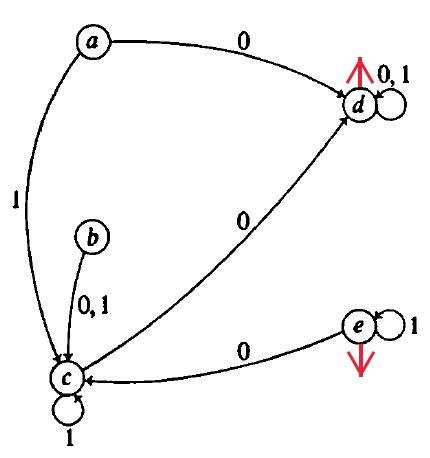
\includegraphics[scale=0.4] {mini-fa} 
	\begin{tikzpicture}[->,>=stealth',shorten >=1pt,auto,node distance=1.5cm, semithick]
	\tikzstyle{every state}=[minimum size=0.1mm]
	\node[state] (a) {$0$};
	\node[state,accepting] (d) [right of=a] {$3$};
	\node[state] (c) [below of=a] {$2$};
	\node[state] (b) [left of=c] {$1$};
	\node[state,accepting] (e) [right of=c] {$4$};
	\path
	(d) edge [loop above] node {$0,1$} (d)
	(c) edge [loop below] node {$1$} (c)
	(e) edge [loop below] node {$1$} (e)
	(a) edge [] node {$0$} (d)
	(a) edge [swap] node {$1$} (c)
	(b) edge [swap] node {$0,1$} (c)
	(e) edge [] node {$0$} (c)
	(c) edge [] node {$0$} (d)
	;
	\end{tikzpicture}
	\caption{Finite state automaton}
	\label{fig:mini-ex2}
\end{figure}

Partitions:\{ \{0 1 2\} \{3 4\}\}
$Q_0=Q_1=\{3,4\}$
split $Q_0$ w.r.t. ($Q_1$,'1') is invalid.\\
Since $T(\{3,4\},'1') = \{3,4\} = Q^\prime = Q_1$, but $Q^{\prime\prime}=Q_0\setminus Q_0^\prime=\emptyset$ \\
so, split[3] w.r.t. ([3],'1') is invalid.

\begin{lstlisting}

	
	************ DFA
	
	DFA
	Q = [0,5)
	S = { 0 }
	F = { 3  4 }
	Transitions = 
	0->{ '0'->3  '1'->2 }
	1->{ ['0','1']->2 }
	2->{ '0'->3  '1'->2 }
	3->{ ['0','1']->3 }
	4->{ '0'->2  '1'->4 }
	
	current = -1
	
	is the DFA Usefulf ?: 1
	
	The combination for all the out labels of State'súC = { '0'  '1' }
	L:
	0 1 2 3 4
	0 0 0 0 0
	Initialize partitions, E0:
	StateEqRel
	{ 0  1  2 }
	{ 3  4 }
	
	Initialize L repr = {F}:
	{ 3 }
	L:
	0 1 2 3 4
	0 0 0 2 0
	=========================== Iterate: k = 1
	L:
	0 1 2 3 4
	0 0 0 1 0
	Partitions:
	StateEqRel
	{ 0  1  2 }
	{ 3  4 }
	
	pick [q] in L:([q],a)=([3],'1')
	split [p] w.r.t ([3],'1')
	===split[0] w.r.t ([3],'1')
	new split of [0] is [-1]
	===split[3] w.r.t ([3],'1')
	new split of [3] is [-1]
	=========================== Iterate: k = 2
	L:
	0 1 2 3 4
	0 0 0 0 0
	Partitions:
	StateEqRel
	{ 0  1  2 }
	{ 3  4 }
	
	pick [q] in L:([q],a)=([3],'0')
	split [p] w.r.t ([3],'0')
	===split[0] w.r.t ([3],'0')
	new split of [0] is [1]
	[p]={ 0  2 }
	[r]={ 1 }
	p and r are the new representatives. Now update L with the smallest of [0] and [1]
	using [r] = [1],L[r]=C.size();
	after update L: 
	L:
	0 1 2 3 4
	0 2 0 0 0
	===split[3] w.r.t ([3],'0')
	new split of [3] is [4]
	[p]={ 3 }
	[r]={ 4 }
	p and r are the new representatives. Now update L with the smallest of [3] and [4]
	using [p] = [3],L[r]=L[p]; L[p]=C.size();
	after update L: 
	L:
	0 1 2 3 4
	0 2 0 2 0
	=========================== Iterate: k = 3
	L:
	0 1 2 3 4
	0 1 0 2 0
	Partitions:
	StateEqRel
	{ 0  2 }
	{ 1 }
	{ 3 }
	{ 4 }
	
	pick [q] in L:([q],a)=([1],'1')
	split [p] w.r.t ([1],'1')
	===split[0] w.r.t ([1],'1')
	new split of [0] is [-1]
	===split[1] w.r.t ([1],'1')
	new split of [1] is [-1]
	===split[3] w.r.t ([1],'1')
	new split of [3] is [-1]
	===split[4] w.r.t ([1],'1')
	new split of [4] is [-1]
	=========================== Iterate: k = 4
	L:
	0 1 2 3 4
	0 0 0 2 0
	Partitions:
	StateEqRel
	{ 0  2 }
	{ 1 }
	{ 3 }
	{ 4 }
	
	pick [q] in L:([q],a)=([1],'0')
	split [p] w.r.t ([1],'0')
	===split[0] w.r.t ([1],'0')
	new split of [0] is [-1]
	===split[1] w.r.t ([1],'0')
	new split of [1] is [-1]
	===split[3] w.r.t ([1],'0')
	new split of [3] is [-1]
	===split[4] w.r.t ([1],'0')
	new split of [4] is [-1]
	=========================== Iterate: k = 5
	L:
	0 1 2 3 4
	0 0 0 1 0
	Partitions:
	StateEqRel
	{ 0  2 }
	{ 1 }
	{ 3 }
	{ 4 }
	
	pick [q] in L:([q],a)=([3],'1')
	split [p] w.r.t ([3],'1')
	===split[0] w.r.t ([3],'1')
	new split of [0] is [-1]
	===split[1] w.r.t ([3],'1')
	new split of [1] is [-1]
	===split[3] w.r.t ([3],'1')
	new split of [3] is [-1]
	===split[4] w.r.t ([3],'1')
	new split of [4] is [-1]
	=========================== Iterate: k = 6
	L:
	0 1 2 3 4
	0 0 0 0 0
	Partitions:
	StateEqRel
	{ 0  2 }
	{ 1 }
	{ 3 }
	{ 4 }
	
	pick [q] in L:([q],a)=([3],'0')
	split [p] w.r.t ([3],'0')
	===split[0] w.r.t ([3],'0')
	new split of [0] is [-1]
	===split[1] w.r.t ([3],'0')
	new split of [1] is [-1]
	===split[3] w.r.t ([3],'0')
	new split of [3] is [-1]
	===split[4] w.r.t ([3],'0')
	new split of [4] is [-1]
	
	************ minDFA
	
	DFA
	Q = [0,4)
	S = { 0 }
	F = { 2  3 }
	Transitions = 
	0->{ '0'->2  '1'->0 }
	1->{ ['0','1']->0 }
	2->{ ['0','1']->2 }
	3->{ '0'->0  '1'->3 }
	
	current = -1
	
\end{lstlisting}	


%%%%%%%%%%%%%%%%%%%%%%%%%%%%%%%%%%%%%%%%%%%%%%%%%%
\begin{thebibliography}{99}
		\bibitem[Hopcroft2008]{Hopcroft2008}
	John E. Hopcroft,Rajeev Motwani,Jeffrey D. Ullman著,孙家骕等译,\textit{自动机理论、语言和计算机导论},Third Edition, 机械工业出版社,2008.7
	
	\bibitem[WATSON93a]{WATSON93a}
	WATSON, B. W. \textit{A taxonomy of finite automata construction algorithms}, Computing Science Note 93/43, Eindhoven University of Technology, The Netherlands, 1993. Available by ftp from ftp.win.tue.nl in pub/techreports/pi.
	
	\bibitem[WATSON93b]{WATSON93b}
	WATSON, B. W. \textit{A taxonomy of finite automata minimization algorithms}, Computing Science Note 93/44, Eindhoven University of Technology, The Netherlands, 1993. Available by ftp from ftp.win.tue.nl in pub/techreports/pi.
	
	\bibitem[WATSON94a]{WATSON94a}
	WATSON, B. W. \textit{An introduction to the FIRE engine: A C++ toolkit for FInite automata and Regular Expressions}, Computing Science Note 94/21, Eindhoven University of Technology, The Netherlands, 1994. Available by ftp from ftp.win.tue.nl in pub/techreports/pi
	
	\bibitem[WATSON94b]{WATSON94b}
	WATSON, B.W. \textit{The design. and implementation of the FIRE engine:	A C++ toolkit for FInite automata and Regular Expressions}, Computing Science Note 94/22, Eindhoven University of Technology, The Netherlands, 1994. Available by ftp from ftp.win.tue.nl in pub/techreports/pi.
	
	\bibitem[Chrison2007]{Chrison2007}
	Christos G. Cassandras and St$\acute{e}$phane Lafortune, \textit{Introduction to Discrete Event Systems},Second Edition,New York,Springer,2007
	
	\bibitem[Wonham2018]{Wonham2018}
	W. M. Wonham and Kai Cai,\textit{Supervisory Control of Discrete-Event Systems}, Revised 2018.01.01
	
	\bibitem[Jean2018]{Jean2018}
	Jean-$\acute{E}$ric Pin, \textit{Mathematical Foundations of Automata Theory},Version of June 15,2018
	
	\bibitem[蒋宗礼2013]{蒋宗礼2013}
	蒋宗礼,姜守旭, \textit{形式语言与自动机理论(第3 版)}, 清华大学出版社,2013.05
	
	
	\bibitem[Lipschutz2007]{Lipschutz2007}
	S. Lipschutz and M. L. Lipson, \textit{Schaum's Outline of Theory and Problems of Discrete Mathematics}, Third Edition, New York: McGraw-Hill, 2007.
	
	\bibitem[Rosen2007]{Rosen2007}
	K. H. Rosen, \textit{Discrete Mathematics and Its Applications}, Seventh Edition, New York: McGraw-Hill, 2007.
	
	\bibitem[R.Su and Wonham2004]{R.Su and Wonham2004}
	R. Su and W. M. Wonham, \textit{Supervisor reduction for discrete-event systems}, Discrete Event Dyn. Syst., vol. 14, no. 1, pp. 31–53, Jan. 2004.
	
	\bibitem[Hopcroft71]{Hopcroft71}
	Hopcroft, J.E. \textit{An n log n algorithm for minimizing states in a finite automaton}, in The Theory of Machines and Computations (Z. Kohavi, ed.), pp.180-196, Academic Press, New York, 1971.
	
	\bibitem[Gries73]{Gries73}
	Gries, D. \textit{Describing an Algorithm by Hopcroft}, Acta Inf. 2:97 109, 173. $\copyright$ by Springer-Verlag 1973
	
	\bibitem[Knuutila2001]{Knuutila2001}
	Knuutila, T. \textit{Re-describing an Algorithm by Hopcroft}. Theoret. Computer Science 250 (2001) 333--363.
	
	\bibitem[Ratnesh95]{Ratnesh95}
	Ratnesh Kumar, \textit{Modeling and Control of Logical Discrete Event Systems}, $\copyright$ 1995 by Springer Science+Business Media New York.
	
	\bibitem[Jean2011]{Jean2011}
	Jean Berstel, Luc Boasson, Olivier Carton, Isabelle Fagnot
	, \textit{Minimization of automata}, Universit$\acute{e}$ Paris-Est Marne-la-Vall$\acute{e}$e 2010 Mathematics Subject Classification: 68Q45, 2011.
	
	\bibitem[Kenneth2012]{Kenneth2012}
	Kenneth H. Rosen著,徐六通译, \textit{离散数学及其应用Discrete Mathematics and Its Applications},seventh Edition, 2012, 机械工业出版社, 北京, 2014.
	
\end{thebibliography}
